\documentclass[handout]{beamer}

\usetheme[progressbar=frametitle]{metropolis}
\usepackage{appendixnumberbeamer}
\usepackage{booktabs}
\usepackage{amsmath}
\usepackage{amssymb}
\usepackage{tcolorbox}
\usepackage{tikz}
\usepackage{multirow}
\usepackage{listings}

\lstset{
    language=Python,
    basicstyle=\ttfamily\scriptsize,
    keywordstyle=\color{blue},
    stringstyle=\color{orange},
    commentstyle=\color{green!70!black},
    breaklines=true,
    showstringspaces=false,
    tabsize=1,
}


\tcbset{
    colback=white,
    colframe=black!70,
    sharp corners,
    boxrule=0.5pt,
    left=0pt,
    right=0pt,
    top=0pt,
    bottom=0pt,
    boxsep=1pt,
}

\definecolor{metropolisblue}{RGB}{39, 59, 94}



% Begin document
\begin{document}

% Title page
\title{Calculus}
\author{Nipun Batra}
\date{\today}
\institute{IIT Gandhinagar}
\maketitle

\begin{frame}{Derivative}
The derivative of a function of a real variable measures the sensitivity to change of the function value (output value) with respect to a change in its argument (input value). 

Let us consider a function $f(x) = 3x^2$. The derivative of this function is given by: $f'(x) = 6x$.

For every unit change in $x$, the value of $f(x)$ changes by $6x$.
    
\end{frame}

\begin{frame}[fragile]
    \frametitle{Derivative}
    \begin{columns}[t]
        \column{0.5\textwidth}
        \begin{tcolorbox}
        \textbf{JAX}
        \begin{lstlisting}[language=Python, linewidth=\textwidth, xleftmargin=-40pt]
        import jax
        import jax.numpy as np
        
        def f(x):
            return 3 * x ** 2
        
        grad_f = jax.grad(f)
        
        x = 2.0
        derivative = grad_f(x)
        
        print("f'(x) =", derivative)
        \end{lstlisting}
        \end{tcolorbox}
        
        \column{0.5\textwidth}
        \begin{tcolorbox}
        \textbf{Torch}
        \begin{lstlisting}[language=Python, linewidth=\textwidth, xleftmargin=-40pt]
        import torch
        
        def f(x):
            return 3 * x ** 2
        
        x = torch.tensor(2.0, requires_grad=True)
        y = f(x)
        
        y.backward()
        derivative = x.grad
        
        print("f'(x) =", derivative)
        \end{lstlisting}
        \end{tcolorbox}
        \end{columns}
    \end{frame}

\begin{frame}{Partial Derivative}
The partial derivative of a function of several variables is its derivative with respect to one of those variables, with the others held constant (as opposed to the total derivative, in which all variables are allowed to vary).

Let us assume a function $f(x,y) = 2x^2 + 3y$. The partial derivative of this function with respect to $x$ is given by: $\frac{\partial f}{\partial x} = 4x$ and with respect to $y$ is given by: $\frac{\partial f}{\partial y} = 3$.

\end{frame}

\begin{frame}[fragile]
    \frametitle{Partial Derivative}
    
    \begin{columns}[t]
    \column{0.5\textwidth}
    \begin{tcolorbox}
    \textbf{JAX}
    \begin{lstlisting}[language=Python, linewidth=\textwidth, xleftmargin=-20pt]
    f = lambda x, y: 2 * x ** 2 + 3 * y
    
    grad_f_x = jax.grad(f, argnums=0)
    grad_f_y = jax.grad(f, argnums=1)
    
    x = 2.0
    y = 1.5
    
    derivative_x = grad_f_x(x, y)
    derivative_y = grad_f_y(x, y)
    
    print("df/dx =", derivative_x)
    print("df/dy =", derivative_y)
    \end{lstlisting}
    \end{tcolorbox}
    
    \column{0.5\textwidth}
    \begin{tcolorbox}
    \textbf{Torch}
    \begin{lstlisting}[language=Python, linewidth=\textwidth, xleftmargin=-20pt]
    f = lambda x, y: 2 * x ** 2 + 3 * y
    
    x = torch.tensor(2.0, requires_grad=True)
    y = torch.tensor(1.5, requires_grad=True)
    z = f(x, y)
    
    z.backward()
    
    derivative_x = x.grad
    derivative_y = y.grad
    
    print("df/dx =", derivative_x)
    print("df/dy =", derivative_y)
    \end{lstlisting}
    \end{tcolorbox}
    \end{columns}
    \end{frame}
    

\begin{frame}{Gradient}
The gradient is a multi-variable generalization of the derivative. While a derivative can be defined on functions of a single variable, for functions of several variables, the gradient takes its place. The gradient is a vector-valued function, as opposed to a derivative, which is scalar-valued.

Let us assume a function $f(x,y) = 2x^2 + 3y$. The gradient of this function is given by: $\nabla f = \begin{bmatrix} 4x \\ 3 \end{bmatrix}$.
    
\end{frame}

\begin{frame}[fragile]
    \frametitle{Gradient}
    
    \begin{columns}[t]
    \column{0.5\textwidth}
    \begin{tcolorbox}
    \textbf{JAX}
    \begin{lstlisting}[language=Python, linewidth=\textwidth, xleftmargin=-20pt]
    f = lambda x, y: 2 * x ** 2 + 3 * y
    
    grad_f = jax.grad(f, argnums=[0, 1])
    
    x = 2.0
    y = 1.5
    
    gradient = grad_f(x, y)
    
    print("Gradient =", gradient)
    \end{lstlisting}
    \end{tcolorbox}
    
    \column{0.5\textwidth}
    \begin{tcolorbox}
    \textbf{Torch}
    \begin{lstlisting}[language=Python, linewidth=\textwidth, xleftmargin=-20pt]
    f = lambda x, y: 2 * x ** 2 + 3 * y
    
    x = torch.tensor(2.0, requires_grad=True)
    y = torch.tensor(1.5, requires_grad=True)
    
    z = f(x, y)
    z.backward()
    
    gradient = torch.tensor([x.grad, y.grad])
    
    print("Gradient =", gradient)
    tensor([8., 3.])
    \end{lstlisting}
    \end{tcolorbox}
    \end{columns}
    \end{frame}
    

\begin{frame}{Jacobian}
    The Jacobian is a matrix that contains the partial derivatives of a vector-valued function with respect to its input variables. 
For example, let us consider the vector valued function $F(x, y) = \begin{bmatrix} x^2 + y^2 \\ x - y \end{bmatrix}$. The Jacobian of this function is given by: $J_F = \begin{bmatrix} 2x & 2y \\ 1 & -1 \end{bmatrix}$.

In general Jacobian matrix is given as:
\begin{equation*}
    J_F = \begin{bmatrix} \frac{\partial f_1}{\partial x_1} & \frac{\partial f_1}{\partial x_2} & \dots & \frac{\partial f_1}{\partial x_n} \\ \frac{\partial f_2}{\partial x_1} & \frac{\partial f_2}{\partial x_2} & \dots & \frac{\partial f_2}{\partial x_n} \\ \vdots & \vdots & \ddots & \vdots \\ \frac{\partial f_m}{\partial x_1} & \frac{\partial f_m}{\partial x_2} & \dots & \frac{\partial f_m}{\partial x_n} \end{bmatrix}
\end{equation*}

\end{frame}

\begin{frame}{Hessian}
    The Hessian matrix or Hessian is a square matrix of second-order partial derivatives of a scalar-valued function, or scalar field. It describes the local curvature of a function of many variables.

For example, let us consider the function $f(x, y) = x^2 + y^2$. The Hessian of this function is given by: $H_f = \begin{bmatrix} 2 & 0 \\ 0 & 2 \end{bmatrix}$.

In general Hessian matrix is given as:
\begin{equation*}
    H_f = \begin{bmatrix} \frac{\partial^2 f}{\partial x_1^2} & \frac{\partial^2 f}{\partial x_1 \partial x_2} & \dots & \frac{\partial^2 f}{\partial x_1 \partial x_n} \\ \frac{\partial^2 f}{\partial x_2 \partial x_1} & \frac{\partial^2 f}{\partial x_2^2} & \dots & \frac{\partial^2 f}{\partial x_2 \partial x_n} \\ \vdots & \vdots & \ddots & \vdots \\ \frac{\partial^2 f}{\partial x_n \partial x_1} & \frac{\partial^2 f}{\partial x_n \partial x_2} & \dots & \frac{\partial^2 f}{\partial x_n^2} \end{bmatrix}
\end{equation*}

    
\end{frame}

\begin{frame}{Hessian}
   We can construct the Hessian by taking the Jacobian of the gradient. For example, let us consider the function $f(x, y) = x^2 + y^2$. The gradient of this function is given by: $\nabla f = \begin{bmatrix} 2x \\ 2y \end{bmatrix}$. 

   We can consider the first element in this vector as $\nabla f_1$ and second element as $\nabla f_2$.

   So, the Hessian of this function is given by: $H_f = \begin{bmatrix} \frac{\partial \nabla f_1}{\partial x} & \frac{\partial \nabla f_1}{\partial y} \\ \frac{\partial \nabla f_2}{\partial x} & \frac{\partial \nabla f_2}{\partial y} \end{bmatrix} = \begin{bmatrix} 2 & 0 \\ 0 & 2 \end{bmatrix}$.


\end{frame}

\begin{frame}
    \frametitle{Examples of Differentiation Terms}
  
    \begin{table}[h]
      \centering
      \begin{tabular}{|c|c|c|}
        \hline
        \textbf{Term} & \textbf{Input Example} & \textbf{Output Example} \\
        \hline
        Jacobian & $\mathbf{f}(x, y) = \begin{bmatrix} 2x + y \\ 3x - 2y \end{bmatrix}$ & $\mathbf{J} = \begin{bmatrix} 2 & 1 \\ 3 & -2 \end{bmatrix}$ \\
        \hline
        Hessian & $f(x, y) = x^2 + xy + y^2$ & $\mathbf{H} = \begin{bmatrix} 2 & 1 \\ 1 & 2 \end{bmatrix}$ \\
        \hline
        Derivative & $f(x) = 3x^2$ & $f'(x) = 6x$ \\
        \hline
        Partial Derivative & $f(x, y) = 2x^2 + 3y$ & $\frac{\partial f}{\partial x} = 4x$ \\
        \hline
        Gradient & $f(x, y) = x^2 + y^2$ & $\nabla f(x, y) = \begin{bmatrix} 2x \\ 2y \end{bmatrix}$ \\
        \hline
      \end{tabular}
    \end{table}
  
  \end{frame}

\begin{frame}{Gradient in the context of machine learning}
    Let us assume a simple linear regression model: $y = \theta_0 + \theta_1 x$. We can write this model in the form of a vector as: $y = \begin{bmatrix} \theta_0 & \theta_1 \end{bmatrix} \begin{bmatrix} 1 \\ x \end{bmatrix}$.

    The loss is given by: $L = \frac{1}{2} \sum_{i=1}^n (y_i - \theta_0 - \theta_1 x_i)^2$.

    The loss is a scalar and a function of $\theta_0$ and $\theta_1$. 
    
    The gradient of the loss is given by: $\nabla L = \begin{bmatrix} \frac{\partial L}{\partial \theta_0} \\ \frac{\partial L}{\partial \theta_1} \end{bmatrix} = \begin{bmatrix} \sum_{i=1}^n (y_i - \theta_0 - \theta_1 x_i) \\ \sum_{i=1}^n (y_i - \theta_0 - \theta_1 x_i) x_i \end{bmatrix}$.
We can now use a first-order method like gradient descent to find the optimal values of $\theta_0$ and $\theta_1$ as per:
\begin{equation*}
    \begin{bmatrix} \theta_0 \\ \theta_1 \end{bmatrix} \leftarrow \begin{bmatrix} \theta_0 \\ \theta_1 \end{bmatrix} - \alpha \nabla L
\end{equation*}
    \end{frame}

\begin{frame}{Hessian in the context of machine learning}
    Instead of using a first-order method like gradient descent, we can use a second-order method like Newton's method to find the optimal values of $\theta_0$ and $\theta_1$.

    We can write Hessian $H$ in terms of gradient $\nabla L$ as: $H = \begin{bmatrix} \frac{\partial^2 L}{\partial \theta_0^2} & \frac{\partial^2 L}{\partial \theta_0 \partial \theta_1} \\ \frac{\partial^2 L}{\partial \theta_1 \partial \theta_0} & \frac{\partial^2 L}{\partial \theta_1^2} \end{bmatrix} = \begin{bmatrix} \sum_{i=1}^n 1 & \sum_{i=1}^n x_i \\ \sum_{i=1}^n x_i & \sum_{i=1}^n x_i^2 \end{bmatrix}$.
    Newton's method is given by: $\begin{bmatrix} \theta_0 \\ \theta_1 \end{bmatrix} \leftarrow \begin{bmatrix} \theta_0 \\ \theta_1 \end{bmatrix} - \alpha \begin{bmatrix} \frac{\partial^2 L}{\partial \theta_0^2} & \frac{\partial^2 L}{\partial \theta_0 \partial \theta_1} \\ \frac{\partial^2 L}{\partial \theta_1 \partial \theta_0} & \frac{\partial^2 L}{\partial \theta_1^2} \end{bmatrix}^{-1} \begin{bmatrix} \frac{\partial L}{\partial \theta_0} \\ \frac{\partial L}{\partial \theta_1} \end{bmatrix}$.

    
\end{frame}

\begin{frame}{Jacobian in the context of machine learning}
\begin{figure}
    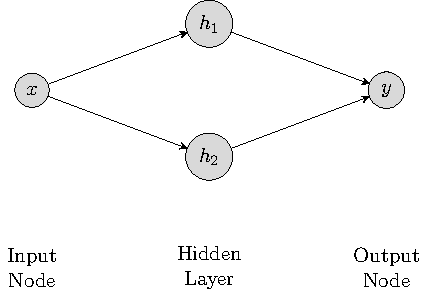
\includegraphics[scale=0.5]{../diagrams/mlp.pdf}
\end{figure}

$h_1 = \mathrm{ReLU}(w_{11} x + b_1)$
$h_2 = \mathrm{ReLU}(w_{12} x + =b_2)$

Now, let us consider the vector $h = \begin{bmatrix} h_1 \\ h_2 \end{bmatrix}$.

The Jacobian of this vector is given by: $J_h = \begin{bmatrix} \frac{\partial h_1}{\partial x} & \frac{\partial h_1}{\partial b_1} & \frac{\partial h_1}{\partial w_{11}} & \frac{\partial h_1}{\partial w_{12}} \\ \frac{\partial h_2}{\partial x} & \frac{\partial h_2}{\partial b_2} & \frac{\partial h_2}{\partial w_{21}} & \frac{\partial h_2}{\partial w_{22}} \end{bmatrix} = \begin{bmatrix} w_{11} & 0 & x & 0 \\ 0 & w_{12} & 0 & x \end{bmatrix}$.

\end{frame}

\end{document}